%!TEX root = ../template.tex
%%%%%%%%%%%%%%%%%%%%%%%%%%%%%%%%%%%%%%%%%%%%%%%%%%%%%%%%%%%%%%%%%%%%
%% chapter5.tex
%% NOVA thesis document file
%%
%% Chapter with lots of dummy text
%%%%%%%%%%%%%%%%%%%%%%%%%%%%%%%%%%%%%%%%%%%%%%%%%%%%%%%%%%%%%%%%%%%%
\chapter{Evaluation}
\label{cha:evaluation}

%\textbf{TOPICS :}
%\begin{itemize}
%	\item Benchmark the iCBD-Replication Module
%	\item Assert the performance gained by storing iMI closer to client workstations
%\end{itemize}

The following chapter reports the experimental work performed in order to study both the executability and performance of the Replication and Caching Service. We describe the tests defined and performed following with some analysis of the results obtained, always trying to co-relate to the effects observed throughout the platform.

The chapter is divided into the following sections:

\begin{description}
    %
    \item [Section~\ref{sec:eval_exp_setup}] .
    %
    \item [Section~\ref{sec:eval_method}] ..
    %
    \item [Section~\ref{sec:eval_rep_bench}] ..
    %
    \item [Section~\ref{sub:eval_cache_bench}] ..
    %
\end{description}

%%-------------------------------------------------------------------
%%	5. - Motivation
%%-------------------------------------------------------------------
%\section{Motivation}
%\label{sec:eval_motivation}

%https://stackoverflow.com/questions/1198691/testing-io-performance-in-linux
%https://dl.acm.org/citation.cfm?id=1367829.1367831

%https://github.com/axboe/fio
%https://github.com/giantswarm/filesystem-benchmark


%%-------------------------------------------------------------------
%%	5. - Experimental Setup
%%-------------------------------------------------------------------
\section{Experimental Setup}
\label{sec:eval_exp_setup}

To ensure the correct execution of all the tests we intended to carry out some adjustments to the iCBD platforms were necessary. To the infrastructure, we deployed two more virtual cache servers (adding to the physical cache server already in operation) with the entire iCBD solution including the RCS. 

Also as discussed in the previous chapter, the Computer Science Department provided two laboratories (Lab 110 and Lab. 112) fully equipped with fifteen machines each (the general specifications of these machines can be seen in the table~\ref{tab:exp_lab_work}), with the objective of performing validation testing of the caching solution at a functional level and then the execution of performance tests.

\begin{table}[]
\centering
\begin{tabular}{ll}
\textbf{CPU} & Intel Core i3-7100 @ 3.90GHz \\
\textbf{Memory} & 8 GB \\
\textbf{Storage} & 275GB SSD \\
\textbf{Ethernet} & 1 Gbps
\end{tabular}
\caption{Specifications of the Laboratories Workstations}
\label{tab:exp_lab_work}
\end{table}

There was also a need to make some changes to VMs that were already deployed, in order to make the laboratories fully functional. First, the VMs iCBD-rw and iCBD-home were connected to the networks of both laboratories configuring the interfaces with fixed IPs. Then, one interface of the iCBD-imgs VM was set up to be connected to the Lab. 110 network and also assigned a fixed IP, then some changes were performed in the iCBD configuration files to allow workstations connected to this network access to iMIs. Also, in the Physical Cache Server, one of the interfaces was configured in the network of Lab. 112, and similar configurations were necessary for this server to provide iMIs to the workstations of this Laboratory.

It is still important to note two aspects, first the Physical Cache Server and the Lab. 112 workstations are attached to the same managed switch, so the communications between them only cross this device. Whereas all communications between workstations of both laboratories and VMs deploy in the cluster travel through various equipment in the FCT NOVA network and therefore may suffer from adverse network conditions entirely out of our control. Second, all of these connections described above are ensured by Gigabit links, either at the level of the network equipment or by the interfaces (virtual or physical) of the servers. A simplistic schematic of all these connections can be found in Figure~\ref{fig:eval_setup}.

\begin{figure}[htbp]
	\centering
	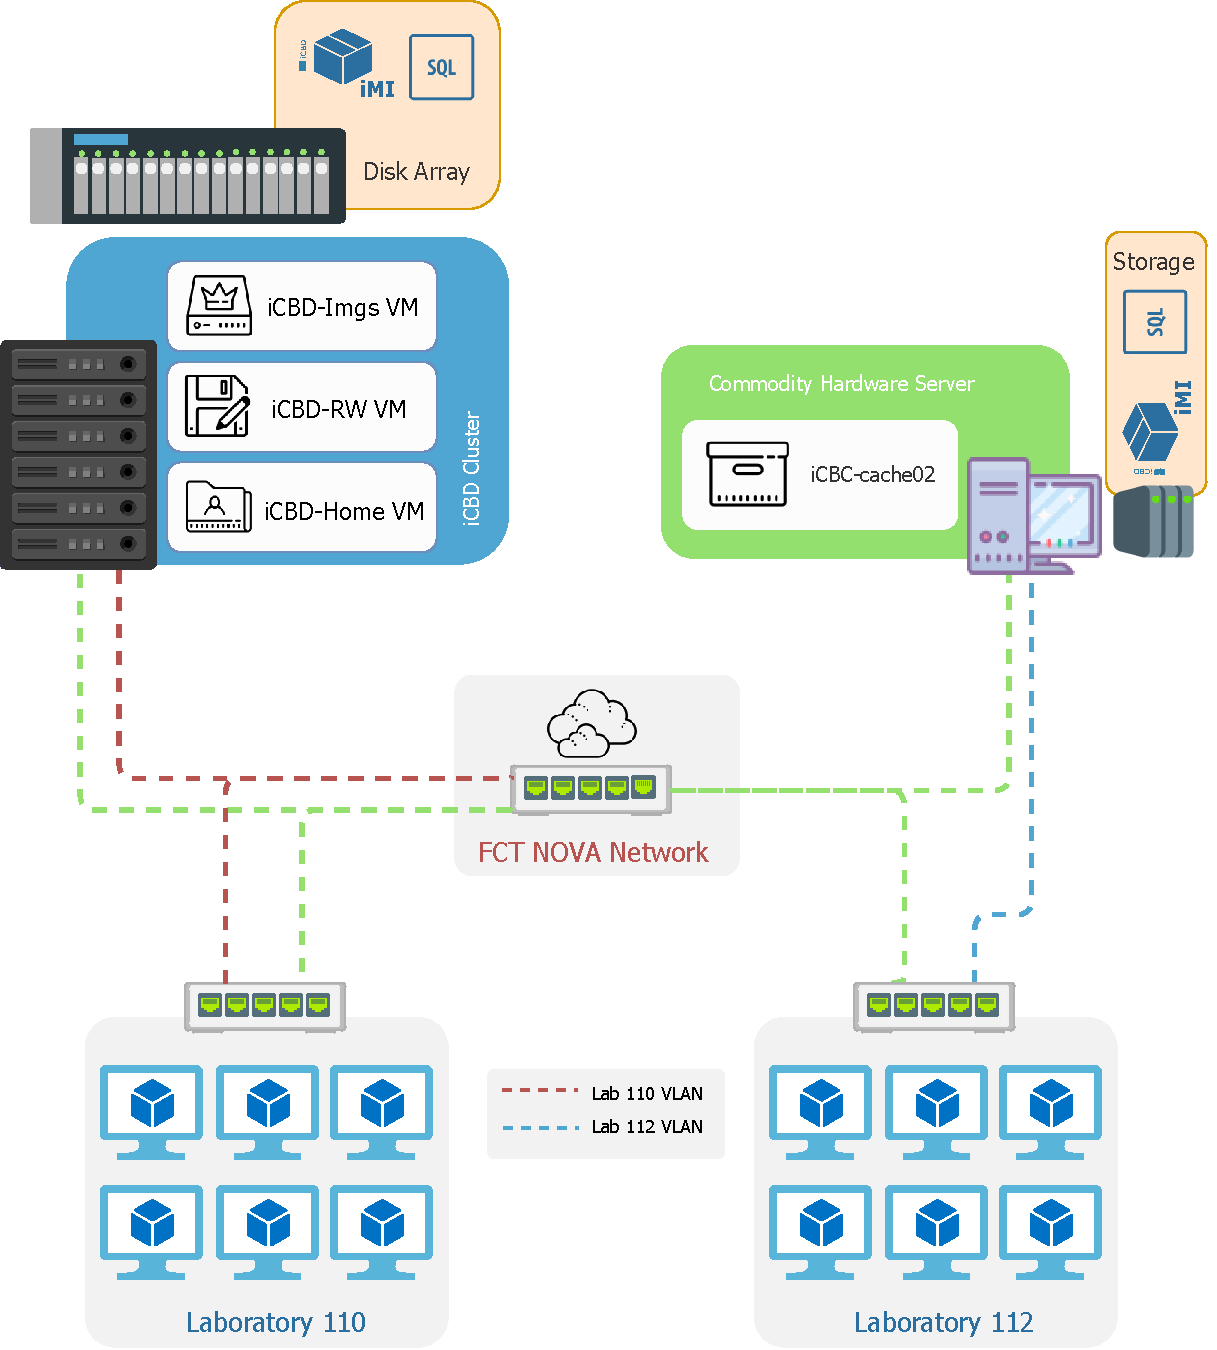
\includegraphics[height=4in]{cap5_lab_setup}
	\caption{iCBD Nodes and Networking Setup}
	\label{fig:eval_setup}
\end{figure}

\begin{table}[htpb]
\centering
\begin{tabular}{lcc}
%\hline
                             & \textbf{FCT NOVA}          & \textbf{SolidNetworks (Development)}              \\ \hline
\textit{\textbf{Servers}}    & 2x HPE ProLiant DL380 Gen9 & 2 x HPE ProLiant DL380 Gen9   \\
\textit{\textbf{Switch}}     & HPE Flexfabric 5700 jg898a & HPE Flexfabric 5700 jg898a    \\
\textit{\textbf{Disk Array}} & HPE MSA 2040 SAN Storage   & N/A - (Storage on the Server) \\
\textit{\textbf{Networking}} & 10 Gbps (between servers)  & 10 Gbps (between servers)     \\ \hline
\end{tabular}
\caption{Physical infrastructure of the FCT NOVA and SolidNetworks sites}
\end{table}


%%-------------------------------------------------------------------
%%	5. - Metodology
%%-------------------------------------------------------------------
\section{Metodology}
\label{sec:eval_method}

The analysis of the RCS was divided into two distinct moments: a first part, which addressed the functional validation of both components of the RCS after being integrated into the iCBD platform, testing its execution correction; and a second part in which we focused on the performance of these components when faced with a production environment.

\paragraph{Functional validation}
\label{par:eval_func_val}

Concerning the replication module, in order to test that this system is functional in a multi-node environment, the Master Node was started in the iCBD-imgs VM and three Replica Nodes, one in each Cache servers (virtual - iCBD-cache01 \& iCBD-Cache03 and physical - iCBD-Cache02). Being observed that the Replica Node had registered on the Name Server as expected and that the communications between the Master Node and Replicas were done correctly.

Next, were carried out two types of test repeatedly. One focused on sending a complete version of an IMI that was not present in the Replicas' Image Repository, forcing the transportation of all the data that are part of this iMIs. We also took advantage of this moment to verify if after the sending process the local Image Repository reflected the addition of the new iMI. This scenario is likely to occur when its the first time that a replica subscribes to a new iMI.

The second type of test revolved about sending versions of iMIs that Replicas already possessed older ones in their repository. This is done to simulate the case where after the administration of an iMI this update is distributed by the Replicas with only the changed data being sent. At the end of each of these tests, we performed a calculation of an MD5 hash with the \texttt{md5sum} tool, in order to ensure that the received data was being reliably transferred.

In order to validate the correct functioning of Cache Servers we mainly focused on iCBD-cache02 (Physical Cache Server), mostly because it was connected directly to one of the laboratories allowing for immediate testing of a workstation iMI boot. Given the integration of the iCBD platform with the remaining network services and policies of  FCT NOVA, a considerable iterative process of experimentation was required, constantly tuning some parameters of some iCBD services until we arrived at a fully functional configuration.
In the end, it was confirmed that it is possible to boot the workstations with iMIs powered by the Cache Server.

\paragraph{Performance Benchmarking}
\label{par:eval_perf_bench}

In this second phase of testing, the goal was to ascertain the performance of RCS in a production environment. In the case of the replication module, we make a comparison between multiple configurations of our solution (with or without compression and secure communications) and the \texttt{rsync} tool, measuring both the time spent on the transference process as well the amount of data transmitted between nodes.

While in the performance tests concerning the cache server, we measured the time spent on the boot process of a workstation. Comparing when the iMI was provided by the Cache Server or by the iCBD-imgs VM hosted at the cluster with more significant resources. For these test batteries, we consider the boot time the time elapsed from the beginning of a load of a kernel until the initialisation of all the services in userspace is finished, making use of the tool \texttt{systemd-analyze}.

Unless stated otherwise, all tests were executed five times removing the best and worst result. The final result is the average of the remaining values. The results of the work performed in these two fields are demonstrated in the following sections.


%%-------------------------------------------------------------------
%%	5. - Replication Service Benchmark
%%-------------------------------------------------------------------
\section{Replication Service Benchmark}
\label{sec:eval_rep_bench}

This benchmark where we want to evaluate the performance of iMI replications within the iCBD platform we idealised two scenarios. One where the full transfer of an iMI to a Replica Node is performed, and the other where the Replica Node already possesses a version of that iMI and only wants to receive the differences (deltas) associated to the new version.

Regarding the IMI used in these tests, a Linux iMI was chosen that contains the Ubuntu 16.04 LTS distribution.  We make use of two sequential versions (v1 and v2) of this iMI in which from one version to the other, during the administration process we applied all the updates proposed by the APT package handling utility. 
We know that the v1 of this iMI stores 38.60GB of data and with the resource to the tool \texttt{btrf-progs} we issued the command \texttt{btrfs filesystem df /path/} giving us the information that from the Btrfs point of view the differences between versions make up 4.45 GB.

For both test scenarios, we produced four sets of settings for the transfer:

\begin{description}
	%
	\item [Rsync] Transfer of an iMI using the rsync tool \footnote{It should be noted that the rsync tool is not aware of a Btrfs subvolume, so the times presented only relate to data transmission, but more operations would be needed to make the iMI functional within the iCBD platform.} with the options \texttt{-r} (recurse into directories); \texttt{-t} (preserve modification times); \texttt{-p} (preserve permissions); \texttt{-l} (copy symlinks as symlinks) and \texttt{-u} (skip files that are newer on the receiver).
	%
	\item [iCBD-Rep - I] Use the iCBD-Replication platform to transfer the iMI using the standard python sockets and no compression.
	%
	\item [iCBD-Rep - II] Apply the iCBD-Replication platform to transfer the iMI using the standard python sockets but compressing the data in a stream with the LZ4 algorithm.
	%
	\item [iCBD-Rep - III] Utilise the iCBD-Replication platform to transfer the iMI using an SSH connection to tunnel the data and not using any compression.
	%
\end{description}

%\subsubsection{Sending a complete version of an iMI}
%\label{susub:eval_iMI_full}

\paragraph{Sending a complete version of an iMI}
\label{par:eval_iMI_full}

In this test that sends a complete iMI, that is all its 38.60GB of data; we can observe that the iCBD platform with its replication module performs similarly on the three sets of settings used. The results are shown in Table~\ref{tab:eval_imifull}. There is a noticeable advantage of the rsync tool which takes less time to perform this process. We believe this happens because it detects that there is no data in the replica and so does not perform its usual block-by-block data comparison routines that are very time consuming and resource wasteful. 

\begin{table}[h]
\centering
\begin{tabular}{lcc}
 & \textbf{Time} & \textbf{Data Sent (MB)} \\ \cline{2-3} 
\textit{\textbf{Rsync}} & 12m23s & 39543 \\
\textit{\textbf{iCBD-Rep - I}} & 17m21s & 38947 \\
\textit{\textbf{iCBD-Rep - II}} & 20m35s & 35572 \\
\textit{\textbf{iCBD-Rep - III}} & 22m55s & 39412
\end{tabular}
\caption{Time spent and data transmitted on transferring a complete iMI from Master to Replica}
\label{tab:eval_imifull}
\end{table}

It can also be observed that even without obtaining more favourable times, the use of compression indicates that the IMI is compressible around 8.6\%, noting that not only the data of the IMI is compressed, as are the instructions generated by the \texttt{send} operation of the Btrfs.
However, the is a caveat, because of the rsync's lack of understanding of the Btrfs internal structure, in the end of the process, the data replicated cannot be automatically made available to users, demanding further operations. While using our tool even though is showing that it takes more time to process the whole iMI, it is guaranteed that once the process is finished the transferred iMI is ready to be made accessible to the workstations. 


%\subsubsection{Sending only the delta between version of an iMI}
%\label{susub:eval_iMI_delta}

\paragraph{Sending only the delta between version of an iMI}
\label{par:eval_iMI_delta}

We now present the results for the evaluation of the process of sending just the differences between the two versions of the chosen iMI. From the outset, one can see the drastic reduction of data transmitted by the network, as expected, only sending the data that was modified between v1 and v2 of the iMI. The results we obtained are shown in Table~\ref{tab:eval_imidelta}.

\begin{table}[h]
\centering
\begin{tabular}{lcc}
 & \textbf{Time} & \textbf{Data Sent (MB)} \\ \cline{2-3} 
\textit{\textbf{Rsync}} & 10m15s & 5964 \\
\textit{\textbf{iCBD-Rep - I}} & 1m47s & 4864 \\
\textit{\textbf{iCBD-Rep - II}} & 2m15s & 4713 \\
\textit{\textbf{iCBD-Rep - III}} & 2m55s & 4902
\end{tabular}
\caption{Time spent and data transmitted on transferring a delta between v1 and v2 of an iMI from Master to Replica}
\label{tab:eval_imidelta}
\end{table}

Our solution using Btrfs send \/ receive operations shows as far superior to rsync's performance on the same data set. Even in the cases where the options of compression or cypher of the data were employed the results did not change dramatically.

%This is an optimum taking into account that these two operations are computationally heavy and therefore in addition to placing more load on the machines that by themselves with the replication process already throw high load values

%\textbf{TOPICS :}
%\begin{itemize}
%	\item Replication with rsync (100 / 1000 mbps)
%	\item Replication with iCBD-Replication - Plain Sockets and No Compression (100 / 1000 mbps)
%	\item Replication with iCBD-Replication - Plain Sockets and LZ4 Compression (100 / 1000 mbps)
%	\item Replication with iCBD-Replication - Plain Sockets and zlib Compression (100 / 1000 mbps)
%	\item Replication with iCBD-Replication - Plain Sockets and snappy Compression (100 / 1000 mbps)
%	\item Replication with iCBD-Replication - SSH and No Compression (100 / 1000 mbps)
%\end{itemize}

%https://stackoverflow.com/questions/5357601/whats-the-difference-between-unit-tests-and-integration-tests

% Unit Test Python
%https://docs.python.org/2/library/unittest.html

%Memory profile of the module
%https://pypi.python.org/pypi/memory_profiler

%%-------------------------------------------------------------------
%%	5. - Cache Server Performance Benchmark
%%-------------------------------------------------------------------
\section{Cache Server Performance Benchmark}
\label{sub:eval_cache_bench}

With this next benchmark we present, we want to evaluate the behaviour of introducing a Cache Server in a production environment. In order to obtain some interesting metrics, two types of tests were carried out, one scenario in which five workstations are sequentially booted, and the second experiments with the extreme case in which all the machines in a laboratory are connected at the same time, creating a situation known as boot storm. For each scenario, we measured the boot times of each workstation, and with a tool called netdata~\cite{netdata} monitored the state of the server at the time it is serving the iMis.

In addition to the two scenarios, there are more variables in play. All tests were performed with all links connected at Gigabit speed. Then every single one was repeated with links limited to 100 Mbps. For this to happen, on the tests referring to the Cache Server, the interface that serves the Lab. 112 was configured at this slower speed. As for the VM that serves the Lab. 110, iCBD-imgs, the type of virtual interface employed does not allow the change of its speed but using the Traffic Shaping feature of the Distributed VSwitch, we managed to limit the bandwidth of the entire PortGroup that refers to this laboratory, in the end reaching the goal.

Lastly, we need to explain the three types of boot tested in this section. The iMI chosen for these tests was the same as mentioned above, a Linux iMI with the Ubuntu 16.04 LTS distribution.

\begin{description}
	%
	\item [Linux Server VDI] In this case, the computation is done on one of the cluster nodes in a diskless VM, simulating a traditional VDI environment, with the particularity of using the iCBD platform's network boot. This variant was born due to its versatility during the development of the platform, since we can connect this VM to any of the networks (internal or labs) and perform tests on its operation.
	%
	\item [Linux iCBD Native] When we talk about this variant, we are addressing the boot of an iMI in a physical workstation in which, in this case, the OS Linux runs natively on top of the hardware, with no kind of resource to virtualisation.
	%
	\item [Linux iCBD VM] This last variant presents an interesting feature since it makes use of two iMIs. In a first phase, it boots as described in the previous point, but with two differences. The booted iMI is of an openSUSE 42.2 \footnote{In this case, any other iMI could be used as a base (including natively run and then virtualised the same iMI), the version  42.2 of openSUSE was chosen because it was the iMI that exhibited the best stability in virtualising any other iMI, throughout the development process.}, and this iMI has installed the VMware Workstation Player serving as a foundation to the next one. When the openSUSE iMI boot process ends, the iMI Ubuntu 16.04 is loaded by VMware Player and is then run on a virtual machine. All this without the user realising that he is using a virtual machine running on a different OS.
		%
\end{description}

\begin{figure}[htbp]
	\centering
	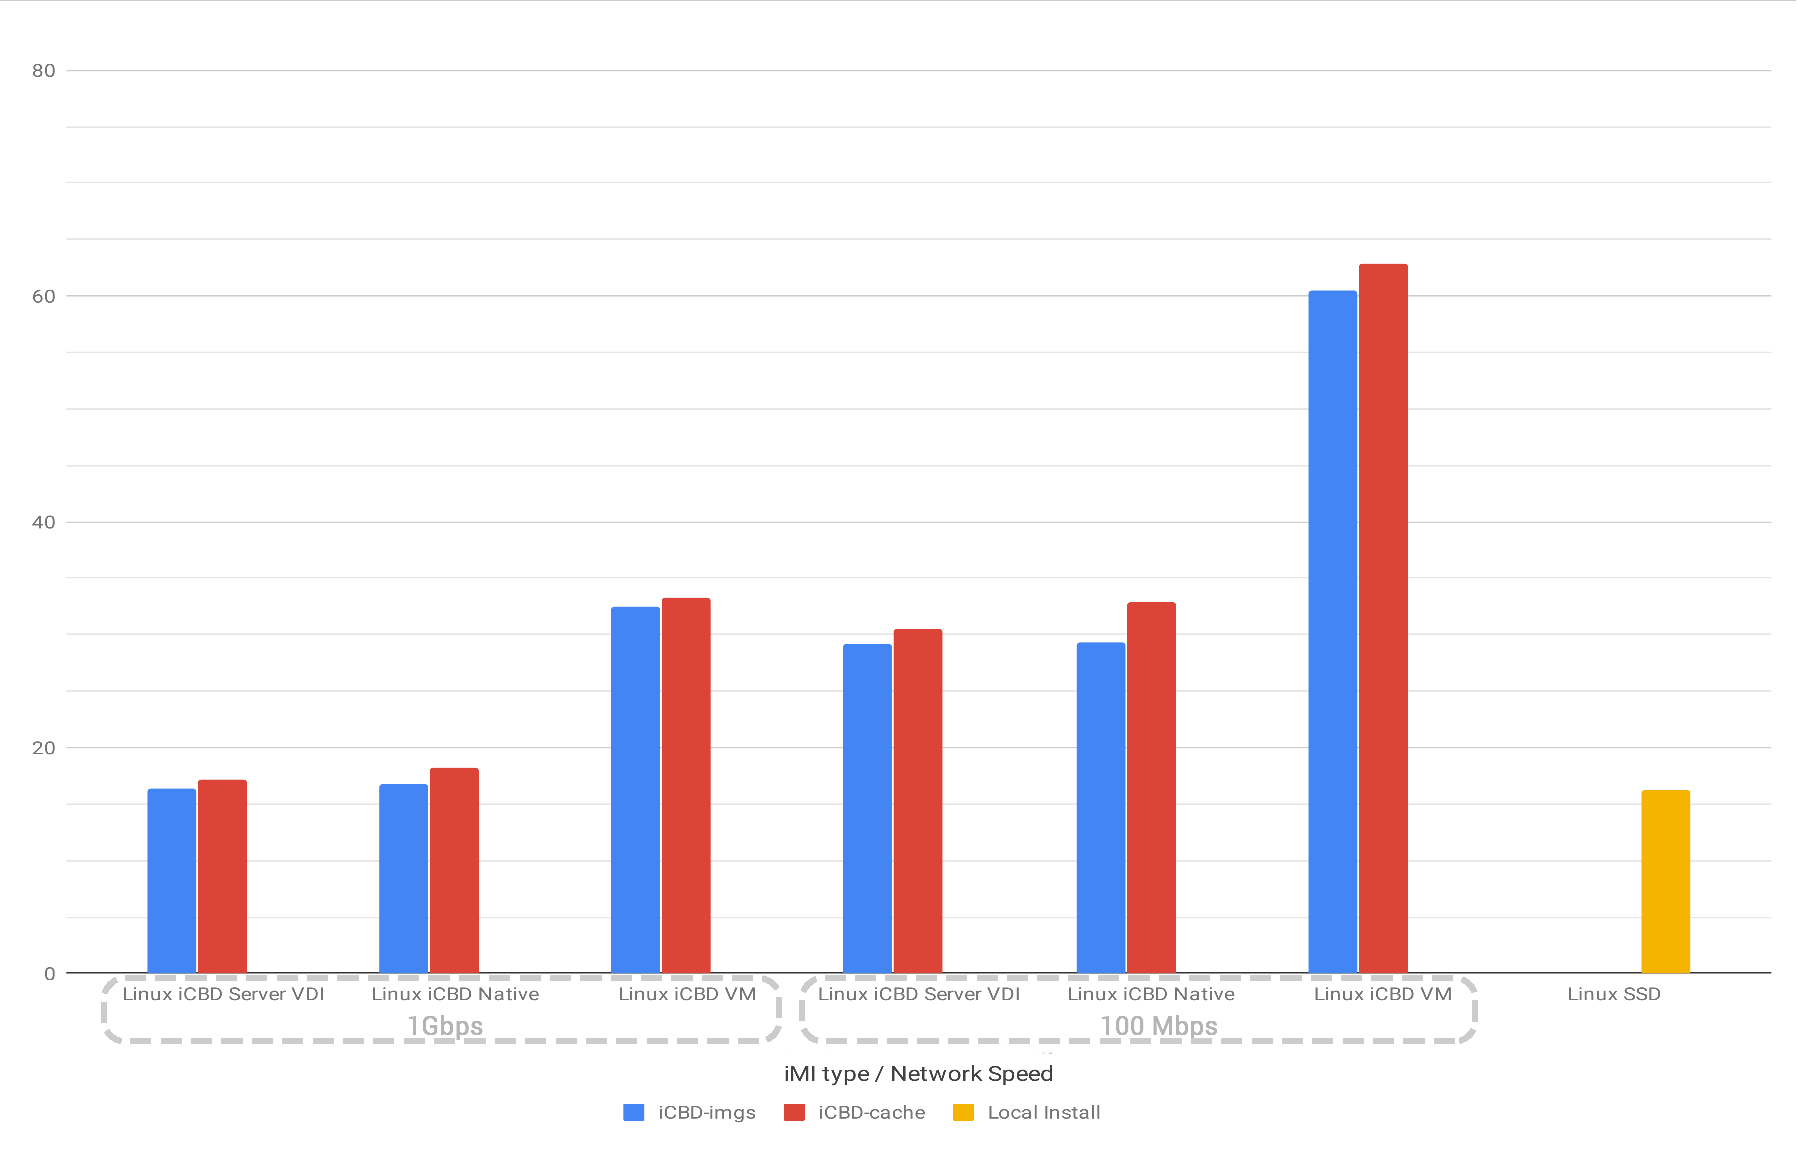
\includegraphics[height=4in]{cap5_NB_iSCSI}
	\caption{Mean Boot Time of five workstations using iSCSI (Sequential Boot Scenario), comparing iMI provider and network speed}
	\label{fig:boot_iscsi}
\end{figure}

\begin{figure}[htbp]
	\centering
	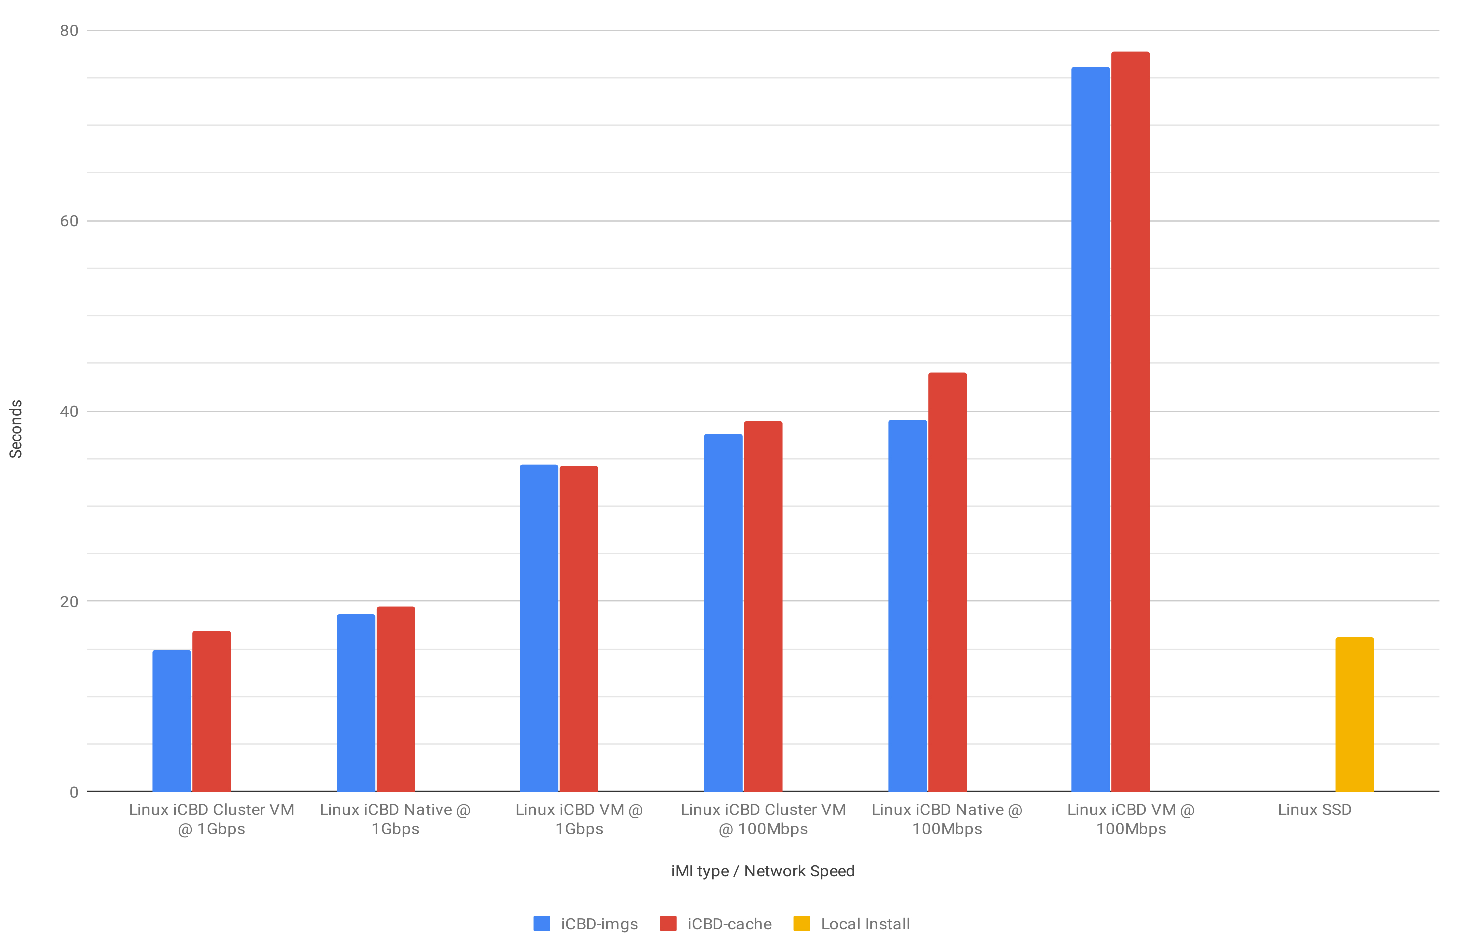
\includegraphics[height=4in]{cap5_NB_NFS}
	\caption{Mean Boot Time of five workstations using NFS (Sequential Boot Scenario), comparing iMI provider and network speed}
	\label{fig:boot_nfs}
\end{figure}

\begin{table}[]
\centering
\begin{tabular}{llcc}
\textbf{iMI} &  & \textbf{iCBD-imgs} & \textbf{iCBD-Cache02} \\ \hline
\multirow{2}{*}{\textit{Linux Server VDI}} & iSCSI & 453.5 MB & 454.3 MB \\
 & NFS & 703.0 MB & 702.1 MB \\ \hline
\multirow{2}{*}{\textit{Linux Client Native}} & iSCSI & 456.3 MB & 453.6 MB \\
 & NFS & 704.2 MB & 703.8 MB \\ \hline
\multirow{2}{*}{\textit{Linux Client VM}} & iSCSI & 834.1 MB & 836.8 MB \\
 & NFS & 950.5 MB & 952.8 MB
\end{tabular}
\caption{Total data received after booting, given each boot variant and for both iMI providers}
\label{tab:boot_totaldata}
\end{table}



%\subsubsection{Benchmark in a Boot Storm condition}
%\label{susub:eval_cache_bootstorm}
\paragraph{Benchmark in a Boot Storm condition}
\label{par:eval_cache_bootstorm}

\begin{table}[]
\centering
\begin{tabular}{llcc}
\textbf{iMI} & \textbf{} & \textbf{iCBD-imgs} & \textbf{iCBD-Cache02} \\ \hline
\multirow{2}{*}{\textit{Linux iCBD Client Native}} & iSCSI & 20.035 s & 23.020 s \\
 & NFS & 23.248 s & 28.156 s \\ \hline
\multirow{2}{*}{\textit{Linux iCBD Client VM}} & iSCSI & 42.627 s & 52.952 s \\
 & NFS & 44.734 s & 54.840 s
\end{tabular}
	\caption{Comparison of boot times in a boot storm situation in both providers (iCBD-imgs and iCBD-cache02)}
	\label{tab:bootstorm_both}
\end{table}


\begin{figure}[htbp]
	\centering
	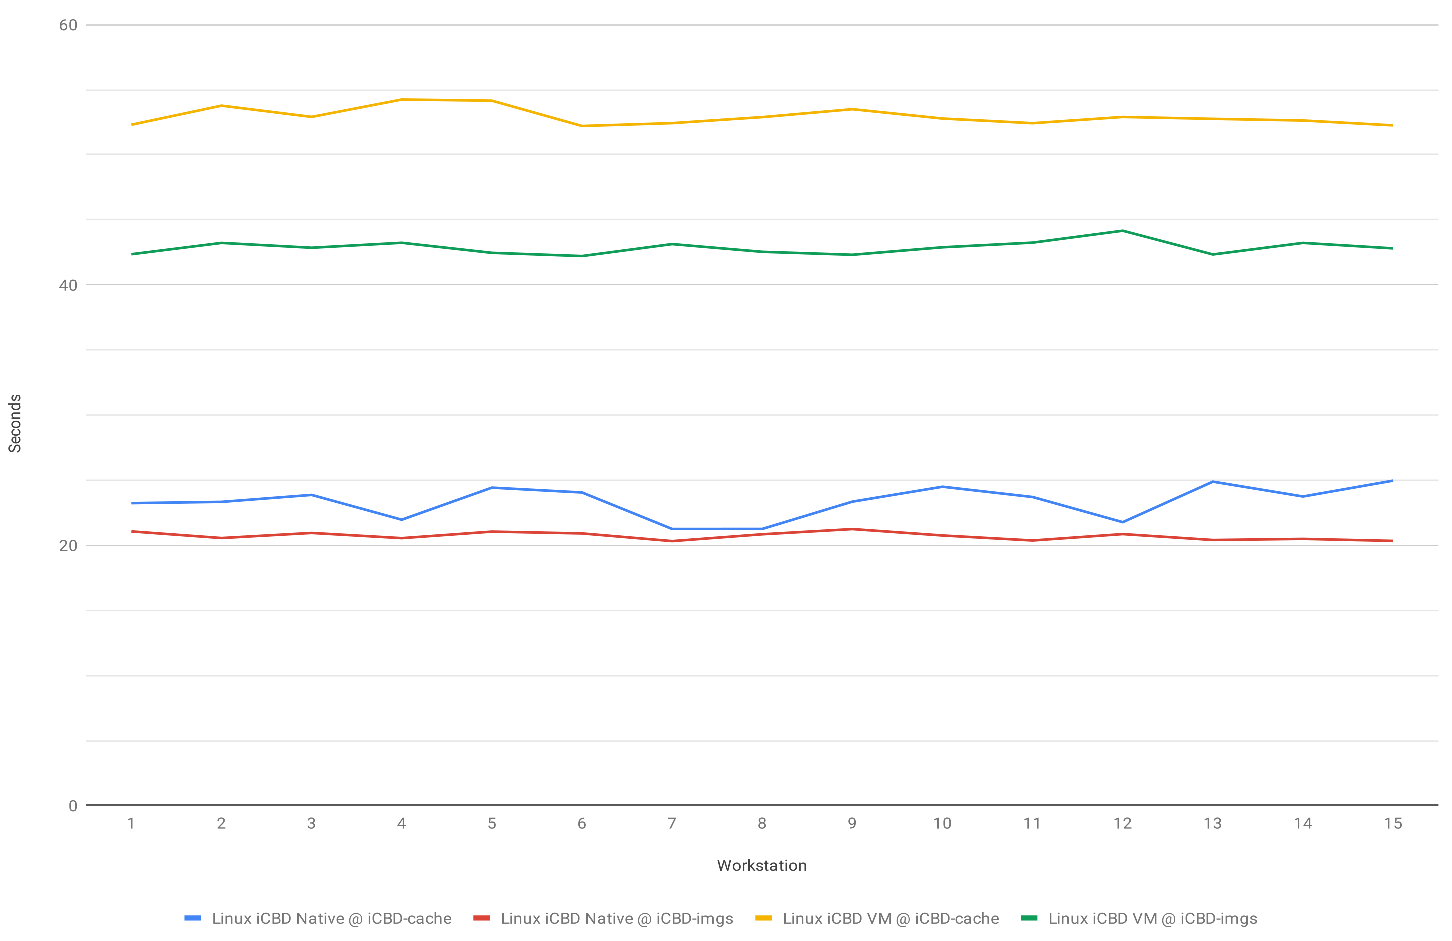
\includegraphics[height=4in]{cap5_BS_combo}
	\caption{Boot Time of fifteen workstations simultaneously (Boot Storm Scenario) comparing iMI provider}
	\label{fig:bootstorm_time}
\end{figure}




%\subsubsection{iMI provider system load}
%\label{susub:eval_sys_load}
\paragraph{iMI provider system load}
\label{par:eval_sys_load}

\begin{figure}[htbp]
	\centering
	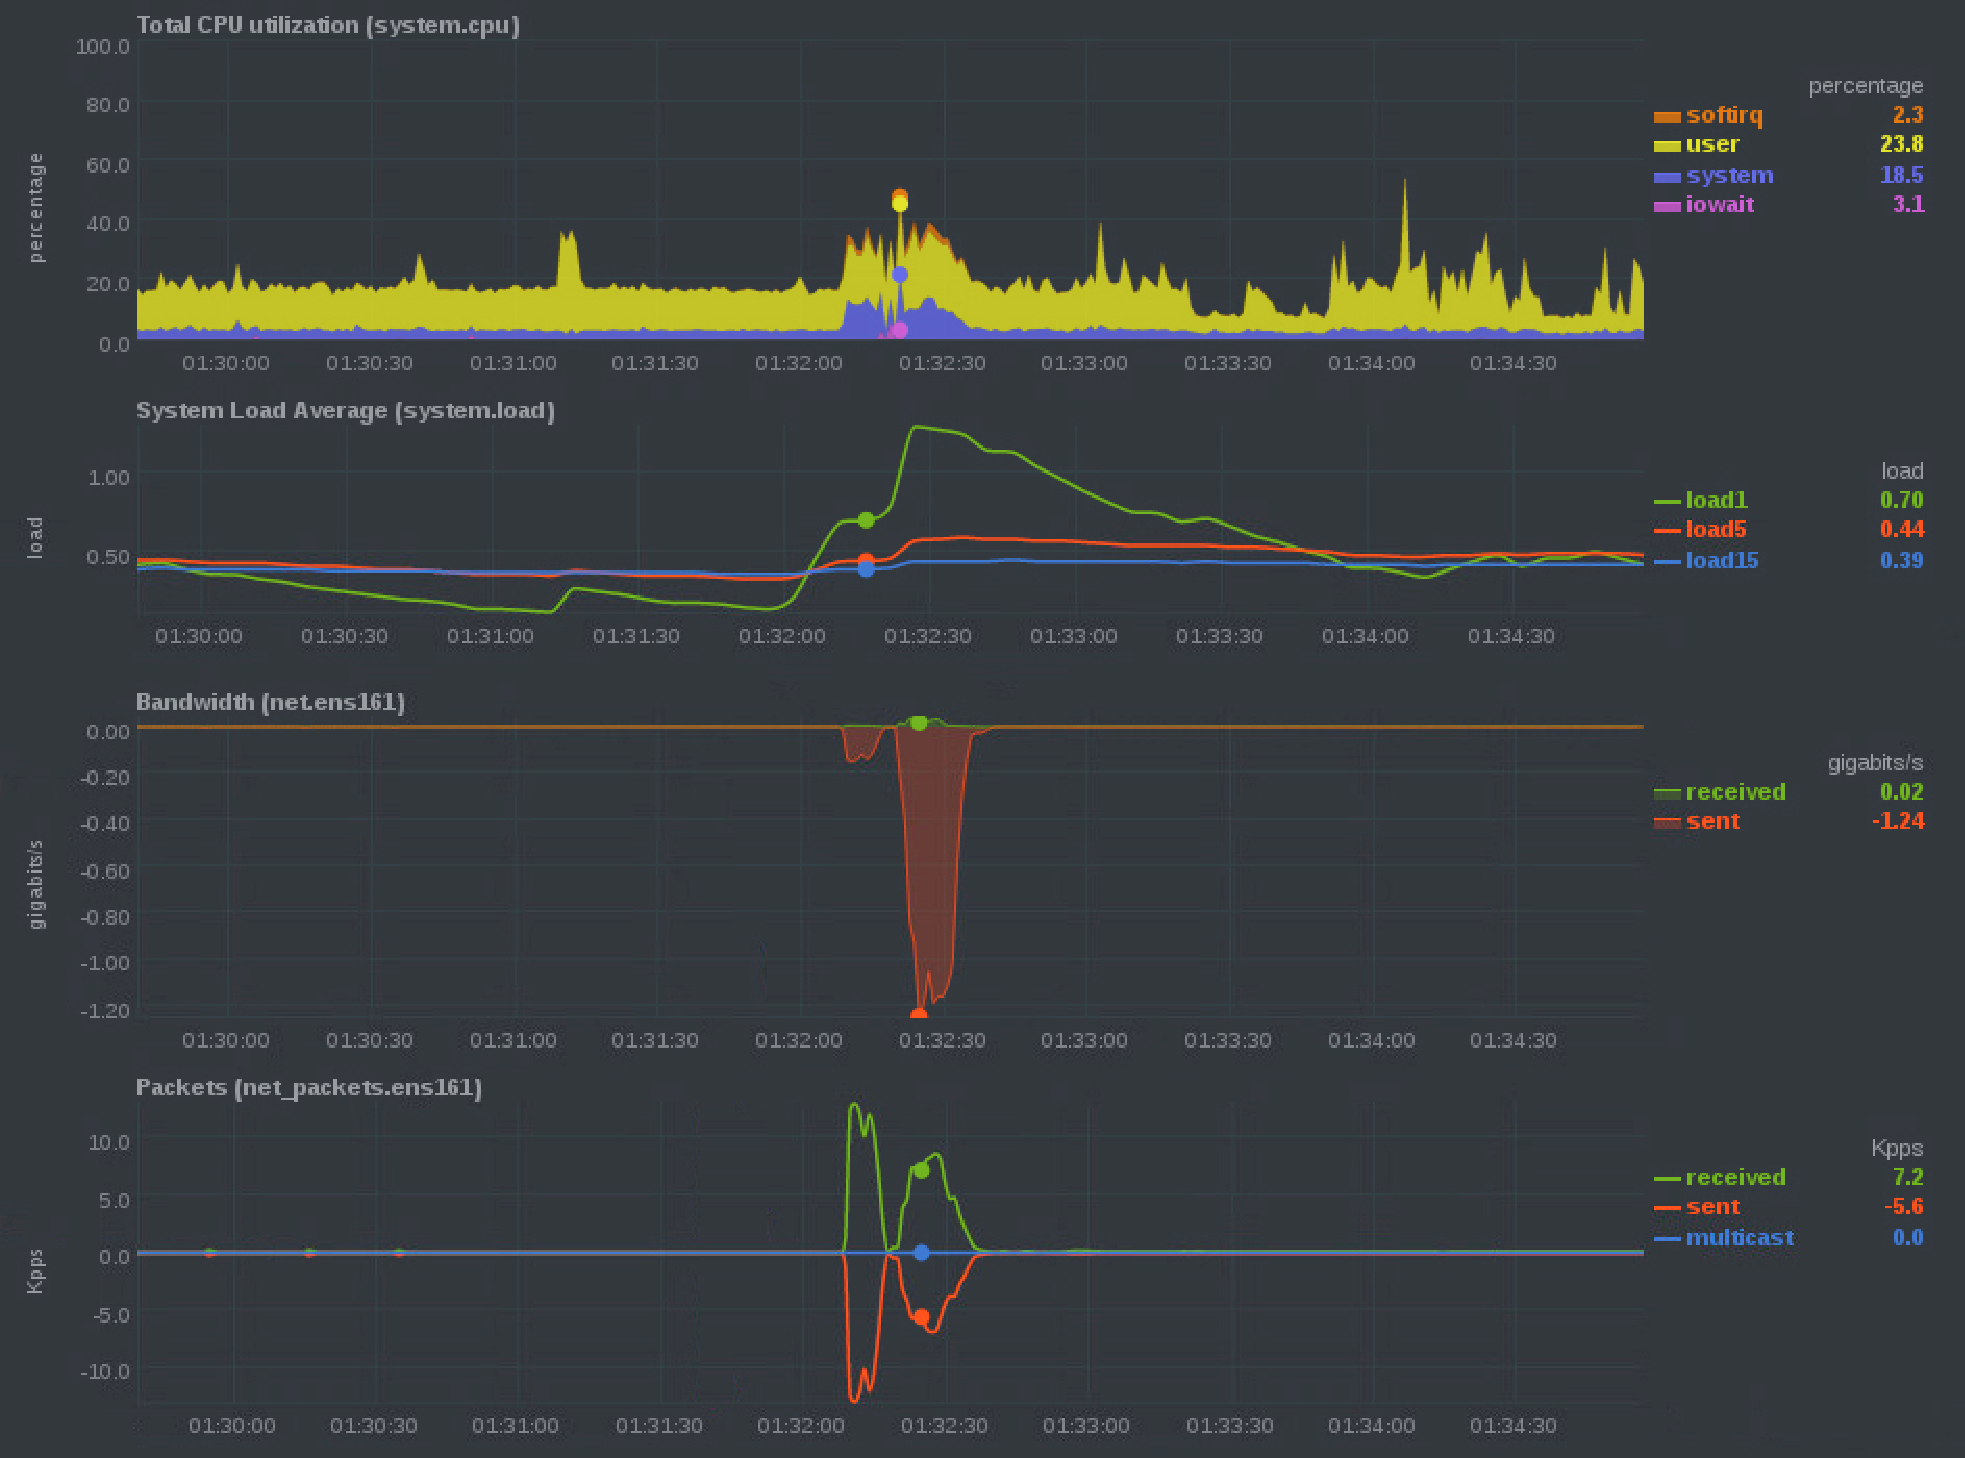
\includegraphics[height=4in]{cap5_secboot_imgs_stats}
	\caption{System metrics for iCBD-imgs on one run of the five workstations sequential boot scenario test}
	\label{fig:boot_imgs_stats}
\end{figure}


\begin{figure}[htbp]
	\centering
	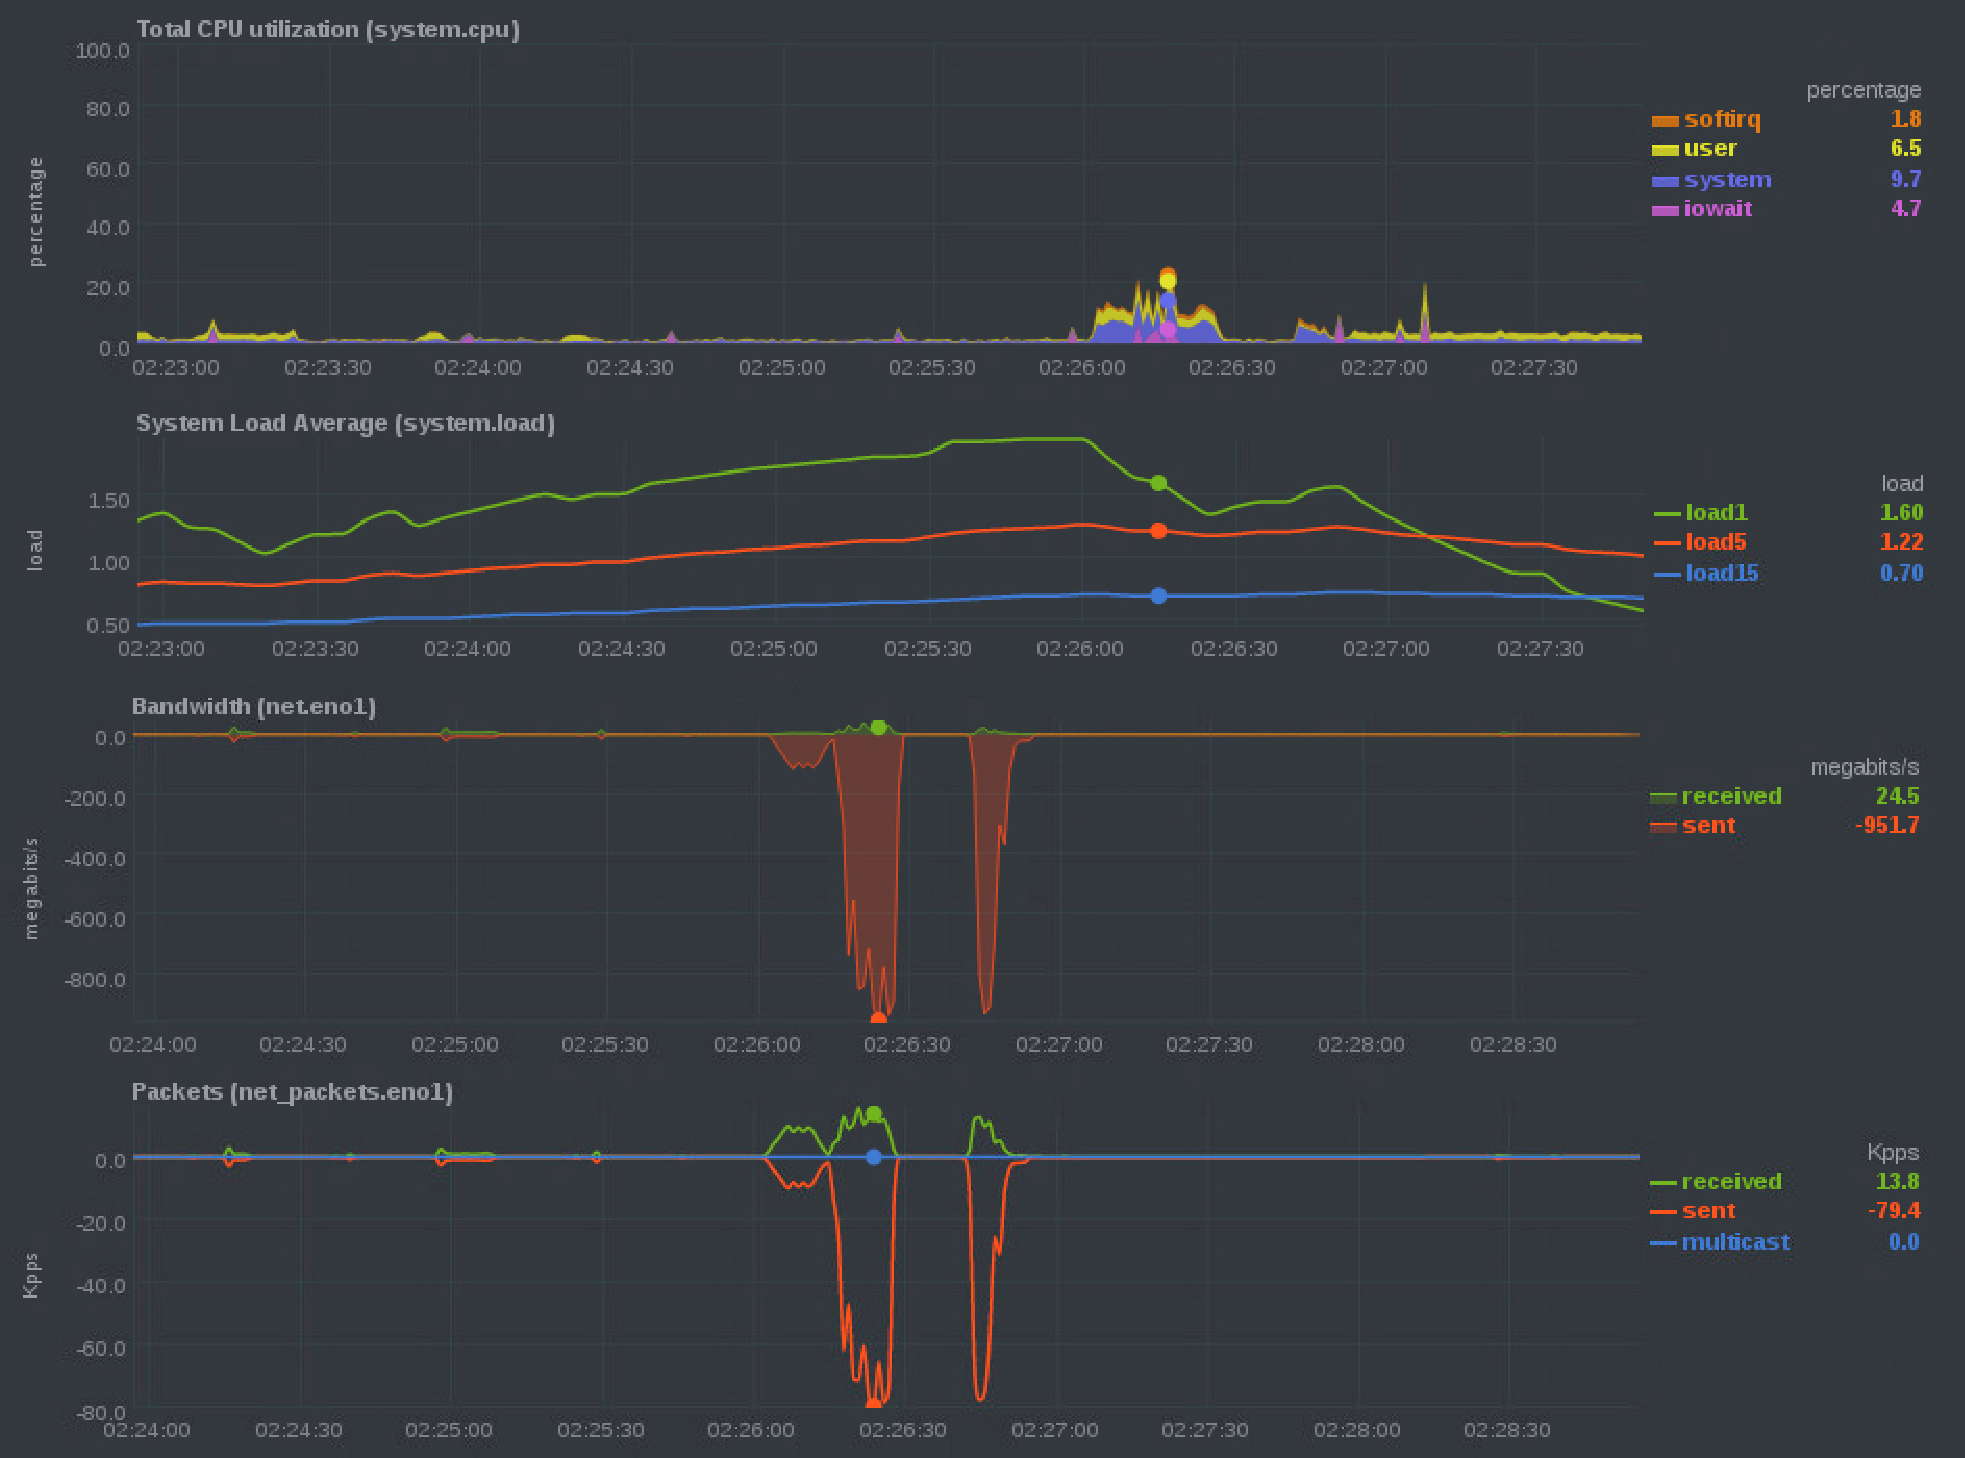
\includegraphics[height=4in]{cap5_secboot_cache_stats}
	\caption{System metrics for iCBD-Cache02 on one run of the five workstations sequential boot scenario test}
	\label{fig:boot_cache_stats}
\end{figure}


\begin{figure}[htbp]
	\centering
	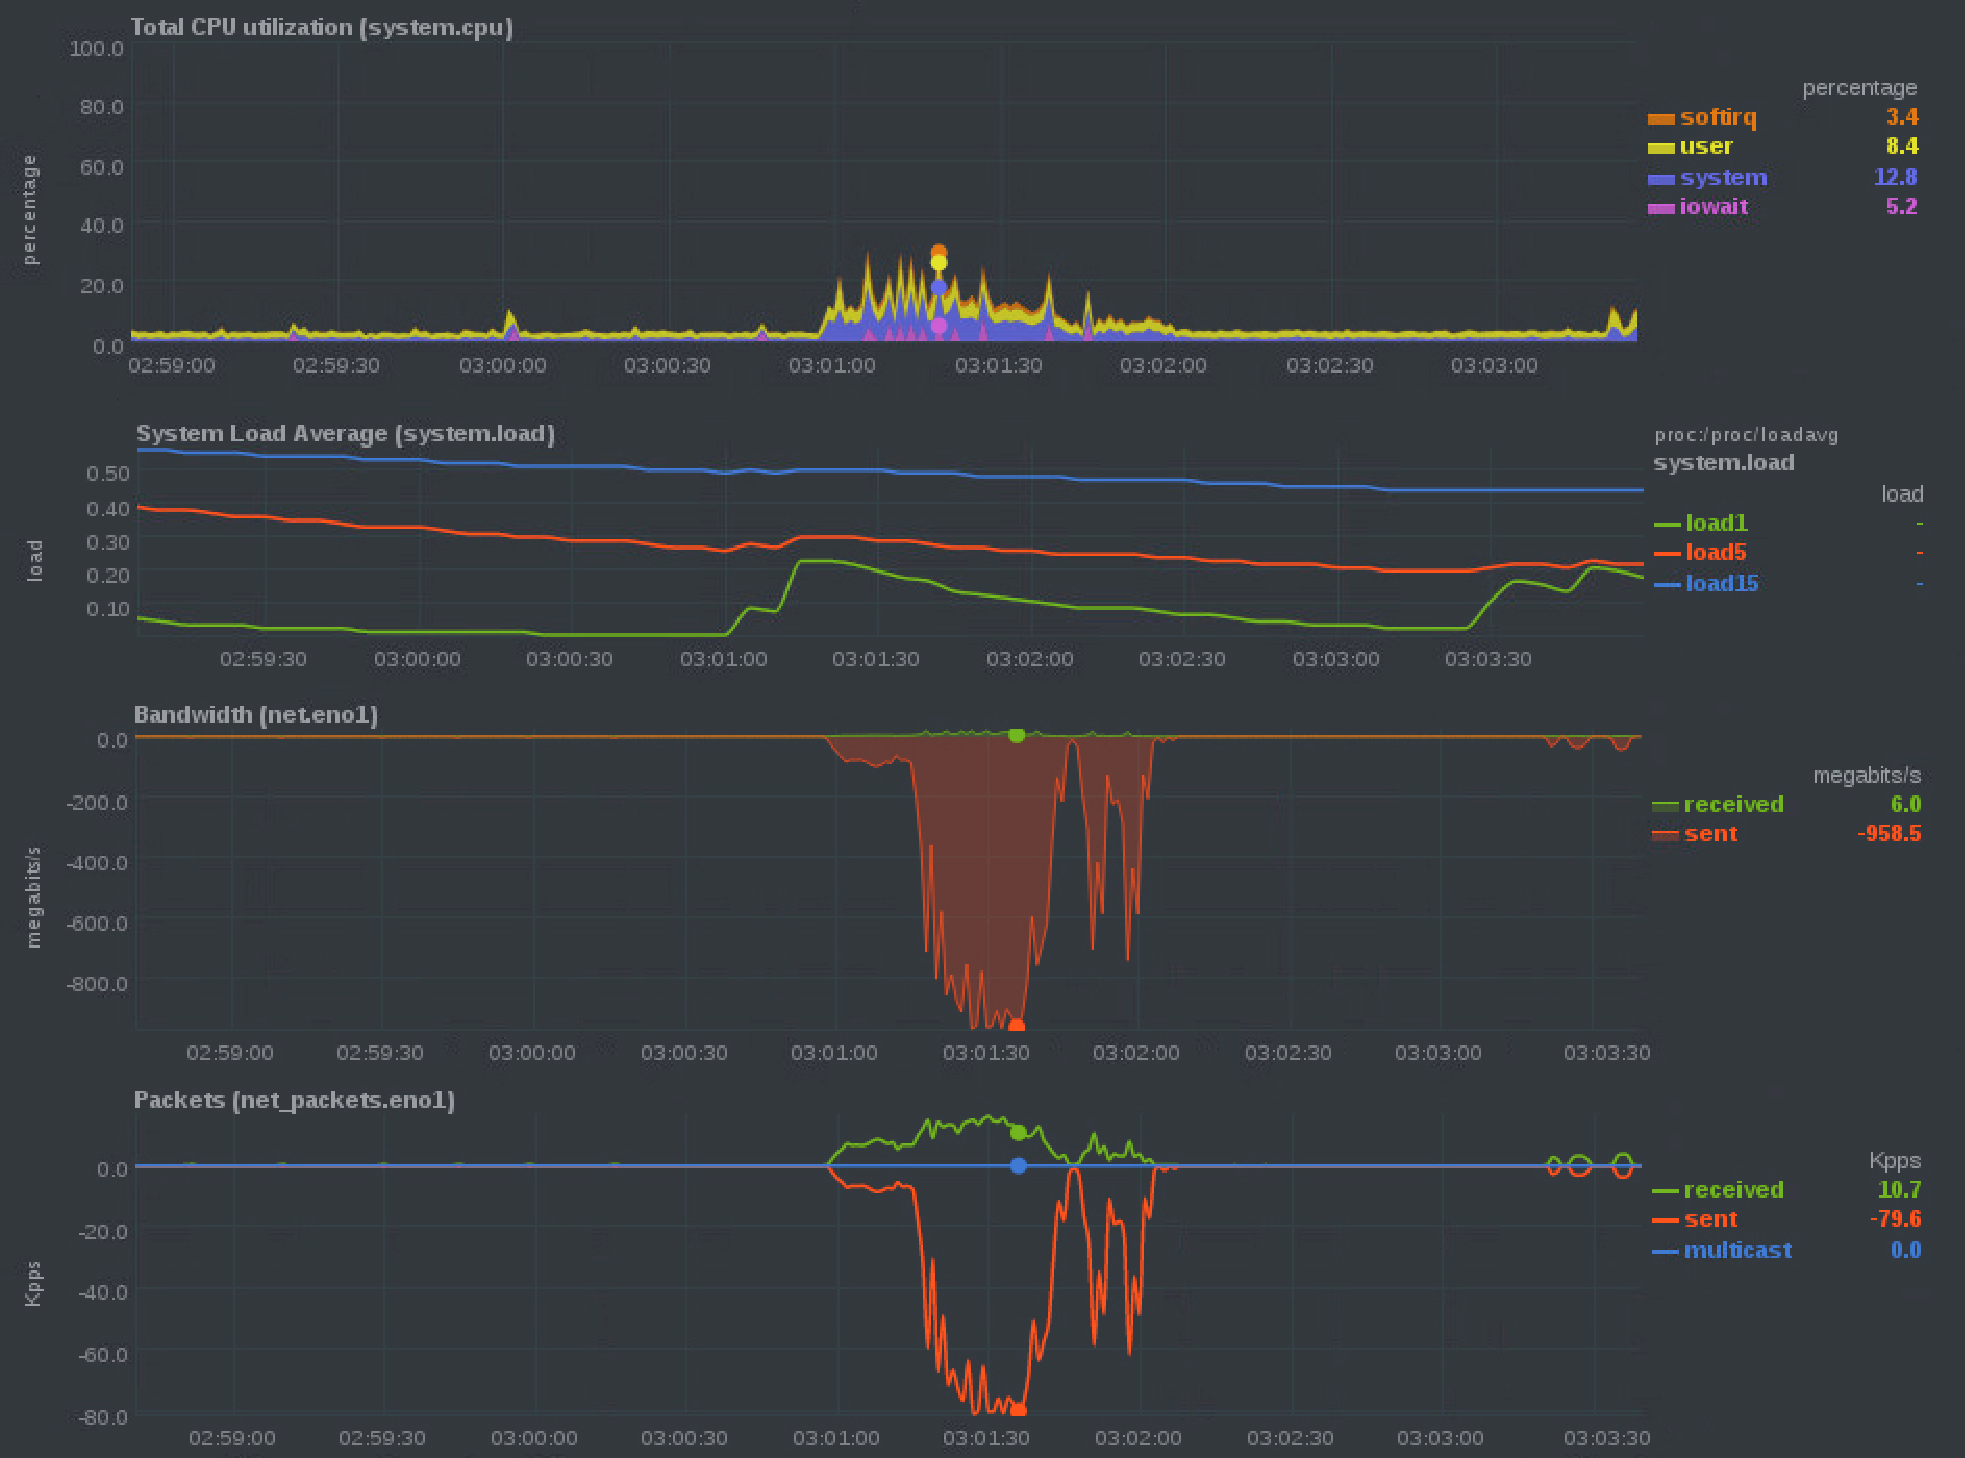
\includegraphics[height=4in]{cap5_bootstorm_cache_stats}
	\caption{System metrics for one run on the iCBD-Cache02 in a boot storm scenario}
	\label{fig:boot_cache_stats}
\end{figure}


%\textbf{TOPICS :}
%\begin{itemize}
%	\item benchmarking 
%	\item Boot time Lab PC
%	\item Boot time iCBD VM in Cluster
%	\item Boot time iCBD in Lab PC (100 / 1000 mbps) iCBD-Imgs VM
%	\item Boot time iCBD in Lab PC (100 / 1000 mbps) iCBD-Cache
%\end{itemize}